%%%% DLI 2026 Submission — IJCAI format

\documentclass{article}
\pdfpagewidth=8.5in
\pdfpageheight=11in

\usepackage{ijcai26}
\usepackage{times}
\usepackage{soul}
\usepackage{url}
\usepackage[hidelinks]{hyperref}
\usepackage[utf8]{inputenc}
\usepackage[small]{caption}
\usepackage{graphicx}
\usepackage{amsmath}
\usepackage{amsthm}
\usepackage{booktabs}
\usepackage{algorithm}
\usepackage{algorithmic}
\usepackage[switch]{lineno}

% Enable line numbers for review submission
\linenumbers

\urlstyle{same}

\pdfinfo{
/TemplateVersion (IJCAI.2026.0)
}

\title{Governance in Practice: A Minimal Schema for Consent and Reuse of Community Data in African Agriculture and Health}

% Anonymous for double-blind review
\author{
Anonymous Author(s)
}

\begin{document}

\maketitle

\begin{abstract}
Community-level datasets in African agriculture and health, from smallholder surveys to local health records, remain underused for data science and machine learning because consent, permitted reuse, and machine-readable metadata are rarely clear. This paper introduces a minimal governance schema that records consent type and scope, permitted use (research, commercial, model training, redistribution), and provenance and audit information. The schema is applied to five recent Africa-related datasets: HarvestStat Africa, LSMS-ISA harmonised, GROW-Africa, Malawi DHS 2024, and HarvestNet (Ethiopia). The paper shows how the schema enables filtering for ethical downstream ML and supports an audit trail for compliance. A reusable template and a Streamlit-based tool are provided for data collectors. The work speaks directly to practical data governance in the age of generative AI, where reuse and training on community data need to be traceable and consent-aware.
\end{abstract}

\section{Introduction}

Data generated by and about communities across Africa is growing rapidly. Smallholder agricultural surveys, household consumption panels, demographic and health surveys, and remote-sensing crop datasets are produced by governments, international organisations, and research groups each year. These datasets hold enormous potential for machine learning applications: crop-yield forecasting, food-security monitoring, disease-burden estimation, and targeted policy design all depend on access to high-quality, representative data \cite{desbureaux2025,gourlay2025,jain2025}. At the same time, the rise of generative AI has created new demand for large-scale training data, raising fresh questions about whether community-level records may be scraped, aggregated, or used in ways their original subjects never envisioned.

Despite this potential, much community-level data in African agriculture and health stays underused. A central reason is that \emph{who} consented to \emph{what}, and \emph{whether} reuse (including model training) is allowed, is seldom documented in a way that downstream users or automated systems can rely on \cite{brown2024,chabilall2024}. Health researchers across sub-Saharan Africa report that unclear consent, worries about commercialisation, and weak governance structures make them hesitant to share data even when they recognise the scientific value \cite{chabilall2024}. Agricultural data collectors face parallel issues: crop-survey microdata is often released under terms that prohibit redistribution or commercial use, but these restrictions are buried in PDF documents or licence pages rather than encoded in a machine-readable form that a data catalogue or ML pipeline could check automatically.

At the same time, normative frameworks around data justice, dynamic consent, and benefit-sharing in African health and agriculture are gaining ground \cite{munung2025,barrett2025}. The African Union's Data Policy Framework and the Malabo Declaration both call for data governance that balances openness with protection. Work on culturally grounded consent has highlighted the importance of multilingual and visual approaches, particularly where participants may speak languages that lack standardised informed-consent templates \cite{omutoko2024}. Yet these frameworks are largely process-oriented: they articulate principles (sovereignty, solidarity, accountability) without specifying how a single dataset should record its governance status in a form that machines can parse.

What is still missing is something concrete at the \emph{dataset} level: minimal, machine-readable documentation of consent, permitted use, and provenance so that (a) data collectors can record governance information in a standard way at the point of collection; (b) downstream users can filter datasets by what is allowed (e.g.\ model training, research only); and (c) auditors can trace who collected what, when, and under what terms.

This paper proposes a \textbf{governance schema} that aims to fill that gap for community-level datasets in African agriculture and health. The schema builds on the idea of Datasheets for Datasets \cite{gebru2021} but adds explicit consent and permitted-use fields that Datasheets do not cover, and it translates concerns from African data governance and ethics literature \cite{munung2025,omutoko2024,brown2024} into machine-readable fields that support filtering and audit. The paper describes the schema design (Section~2), reviews related work (Section~3), applies the schema to five recent Africa-related datasets (Section~4), discusses implications and limitations (Section~5), and concludes with next steps (Section~6). The contribution is practical: a schema definition, a reusable template, rationales for each design choice, five filled governance records, and an open-source Streamlit tool for creating and browsing records.

\section{Related Work}

\subsection{Datasheets, Model Cards, and Dataset Documentation}

Datasheets for Datasets \cite{gebru2021} introduced a structured questionnaire covering motivation, composition, collection process, preprocessing, intended uses, distribution, and maintenance. The framework has become a reference point for responsible dataset release in the ML community. However, Datasheets treat consent and permitted use only indirectly: the questionnaire asks whether data subjects were informed and whether there are legal restrictions, but the answers are free-text narratives rather than machine-readable flags. This makes it difficult to build automated pipelines that filter datasets by governance status.

Model Cards \cite{gebru2021} perform a similar function for trained models, documenting intended use, evaluation metrics, and ethical considerations, but they do not address the upstream question of whether the training data was collected with appropriate consent. Data Nutrition Labels offer a visual summary of dataset characteristics but focus on statistical properties (class balance, missing values) rather than governance metadata. The FAIR principles (Findable, Accessible, Interoperable, Reusable) emphasise metadata quality and interoperability but do not prescribe specific consent or permitted-use fields.

Table~\ref{tab:comparison} summarises what the present schema adds beyond Datasheets for Datasets, highlighting the gap in consent and machine-readable permitted use.

\begin{table}[t]
\centering
\caption{Comparison with Datasheets for Datasets.}
\label{tab:comparison}
\small
\begin{tabular}{@{}p{2.5cm}ll@{}}
\toprule
Aspect & Datasheets & This schema \\
\midrule
Motivation \& composition & Covered & Aligned \\
Recommended uses & Free text & Machine-readable flags \\
Consent type \& scope & Not covered & Required fields \\
Permitted use (ML, commercial, redist.) & Not covered & Yes/no flags \\
Provenance (collector, dates) & Partial & Required + optional \\
Audit (contact, review date) & Not covered & Optional fields \\
\bottomrule
\end{tabular}
\end{table}

\subsection{African Data Governance and Ethics Frameworks}

Several frameworks have emerged from African research communities to address the governance of data generated on the continent. \citeauthor{munung2025}~\shortcite{munung2025} argue for an equity-oriented data-sharing culture built on dynamic consent, benefit-sharing, and data sovereignty, drawing on experiences from large-scale African genomics and health-research initiatives. \citeauthor{barrett2025}~\shortcite{barrett2025} propose an African data ethics framework grounded in decolonial theory, emphasising self-determination, communalist practice, and accountability over frameworks imported from North American or European contexts. \citeauthor{abebe2021}~\shortcite{abebe2021} document narratives and counter-narratives around data sharing in Africa, showing that concerns about exploitation, recolonisation, and benefit extraction shape willingness to share.

On the empirical side, \citeauthor{brown2024}~\shortcite{brown2024} and \citeauthor{chabilall2024}~\shortcite{chabilall2024} surveyed health researchers across sub-Saharan Africa and found that trust and willingness to share depend on clear guidelines and governance, while barriers include unclear consent processes, fear of commercialisation without benefit, and legal gaps in national data-protection regimes. Work on culturally grounded consent \cite{omutoko2024} has highlighted the practical challenges of informed consent in multilingual, low-literacy settings, where standard written consent forms may not be adequate. Policy-level work calls for trustworthy, inclusive data governance for AI in Africa \cite{effoduh2024}, but translating these principles into actionable, dataset-level metadata remains an open problem.

These efforts are largely normative or process-oriented. They articulate what data governance \emph{should} look like, but do not provide a concrete, machine-readable artefact that a data collector can fill in and a downstream ML pipeline can query. The schema presented in this paper targets that gap for community-level datasets in African agriculture and health.

\section{Schema Design}
\label{sec:schema}

The governance schema is organised into five sections: \textbf{identification}, \textbf{consent}, \textbf{permitted use}, \textbf{provenance}, and \textbf{audit}. Each section contains a mix of required and optional fields, designed to be minimal enough that a single data collector can fill in a record in under ten minutes, yet expressive enough to support filtering and audit by downstream users. The schema is distributed as a JSON template with a companion YAML specification; a filled record is a single JSON file that can sit alongside the dataset it describes.

\subsection{Identification}

Each record requires a unique dataset identifier (\texttt{dataset\_id}), a human-readable title, and a domain tag (agriculture, health, or other). An optional geography field records the country or region. These fields align with common dataset documentation practice \cite{gebru2021} and serve as the primary keys for catalogue search. The domain tag was included because governance norms differ between agriculture and health: health data typically requires individual consent and ethics-committee approval, whereas agricultural statistics may rely on institutional agreements.

\subsection{Consent}

The consent section records three required fields and one optional field:

\begin{itemize}
    \item \textbf{consent\_type}: one of \texttt{individual}, \texttt{community}, \texttt{household}, or \texttt{institutional}. This taxonomy reflects the range of consent models observed in African research contexts, from individual informed consent in clinical trials to institutional agreements for aggregate crop statistics.
    \item \textbf{scope}: a free-text description of what participants were told their data would be used for (e.g.\ ``research on crop yields in SSA'').
    \item \textbf{documented}: a boolean indicating whether consent was formally recorded (signed form, audio recording, digital check-box, or similar).
    \item \textbf{consent\_language} (optional): the language(s) in which consent was obtained, addressing the multilingual consent challenges highlighted by \citeauthor{omutoko2024}~\shortcite{omutoko2024}.
\end{itemize}

Datasheets for Datasets do not include any of these fields, yet they are precisely the information a downstream user needs to decide whether a dataset can be used for a given purpose. Making consent type and documentation status machine-readable enables queries such as ``only datasets with documented, individual consent.''

\subsection{Permitted Use}

Four boolean flags indicate whether the following uses are allowed:

\begin{itemize}
    \item \texttt{research}: use for academic or non-profit research.
    \item \texttt{commercial}: use in commercial products or services.
    \item \texttt{model\_training}: use as training data for ML models, including generative AI.
    \item \texttt{redistribution}: sharing the data with third parties.
\end{itemize}

An optional free-text field (\texttt{use\_restrictions}) can record additional conditions (e.g.\ ``DHS registration required''). The \texttt{model\_training} flag was added specifically because the rise of foundation models and generative AI has created a new category of reuse that most existing licence frameworks do not address explicitly. Many datasets released under research-only terms are silent on whether model training counts as research, creating ambiguity that the schema resolves with a dedicated flag. This design turns benefit-sharing and licensing concerns from the literature \cite{munung2025,chabilall2024} into something a data catalogue or ML pipeline can check programmatically.

\subsection{Provenance}

The collecting organisation is required. Collection dates, dataset version, and last-update timestamp are optional but support accountability and reproducibility. These fields overlap with Datasheets but are included here to keep each governance record self-contained, so that a user does not need to consult a separate Datasheet to answer ``who collected this and when?''

\subsection{Audit}

Optional fields for a contact email, a governance-review date, and free-text notes support ongoing stewardship. The contact field gives downstream users a clear ``who to ask'' for governance questions, which survey evidence suggests is a key enabler of trust in data sharing \cite{brown2024,effoduh2024}. The review-date field encourages periodic reassessment of governance status, recognising that consent terms and legal frameworks evolve over time.

\subsection{Tooling}

The schema is accompanied by an open-source Streamlit application that provides two functions: (a) browsing and filtering existing governance records by domain, consent type, or permitted-use flags; and (b) creating new governance records through a guided form. Figure~\ref{fig:tool} shows both interfaces. The tool validates required fields on submission and exports records as JSON files. It is intended for data collectors who may not be comfortable editing JSON directly, and for data users who want to explore governance metadata across multiple datasets without writing code.

\begin{figure*}[t]
\centering
\begin{minipage}{0.48\textwidth}
\centering
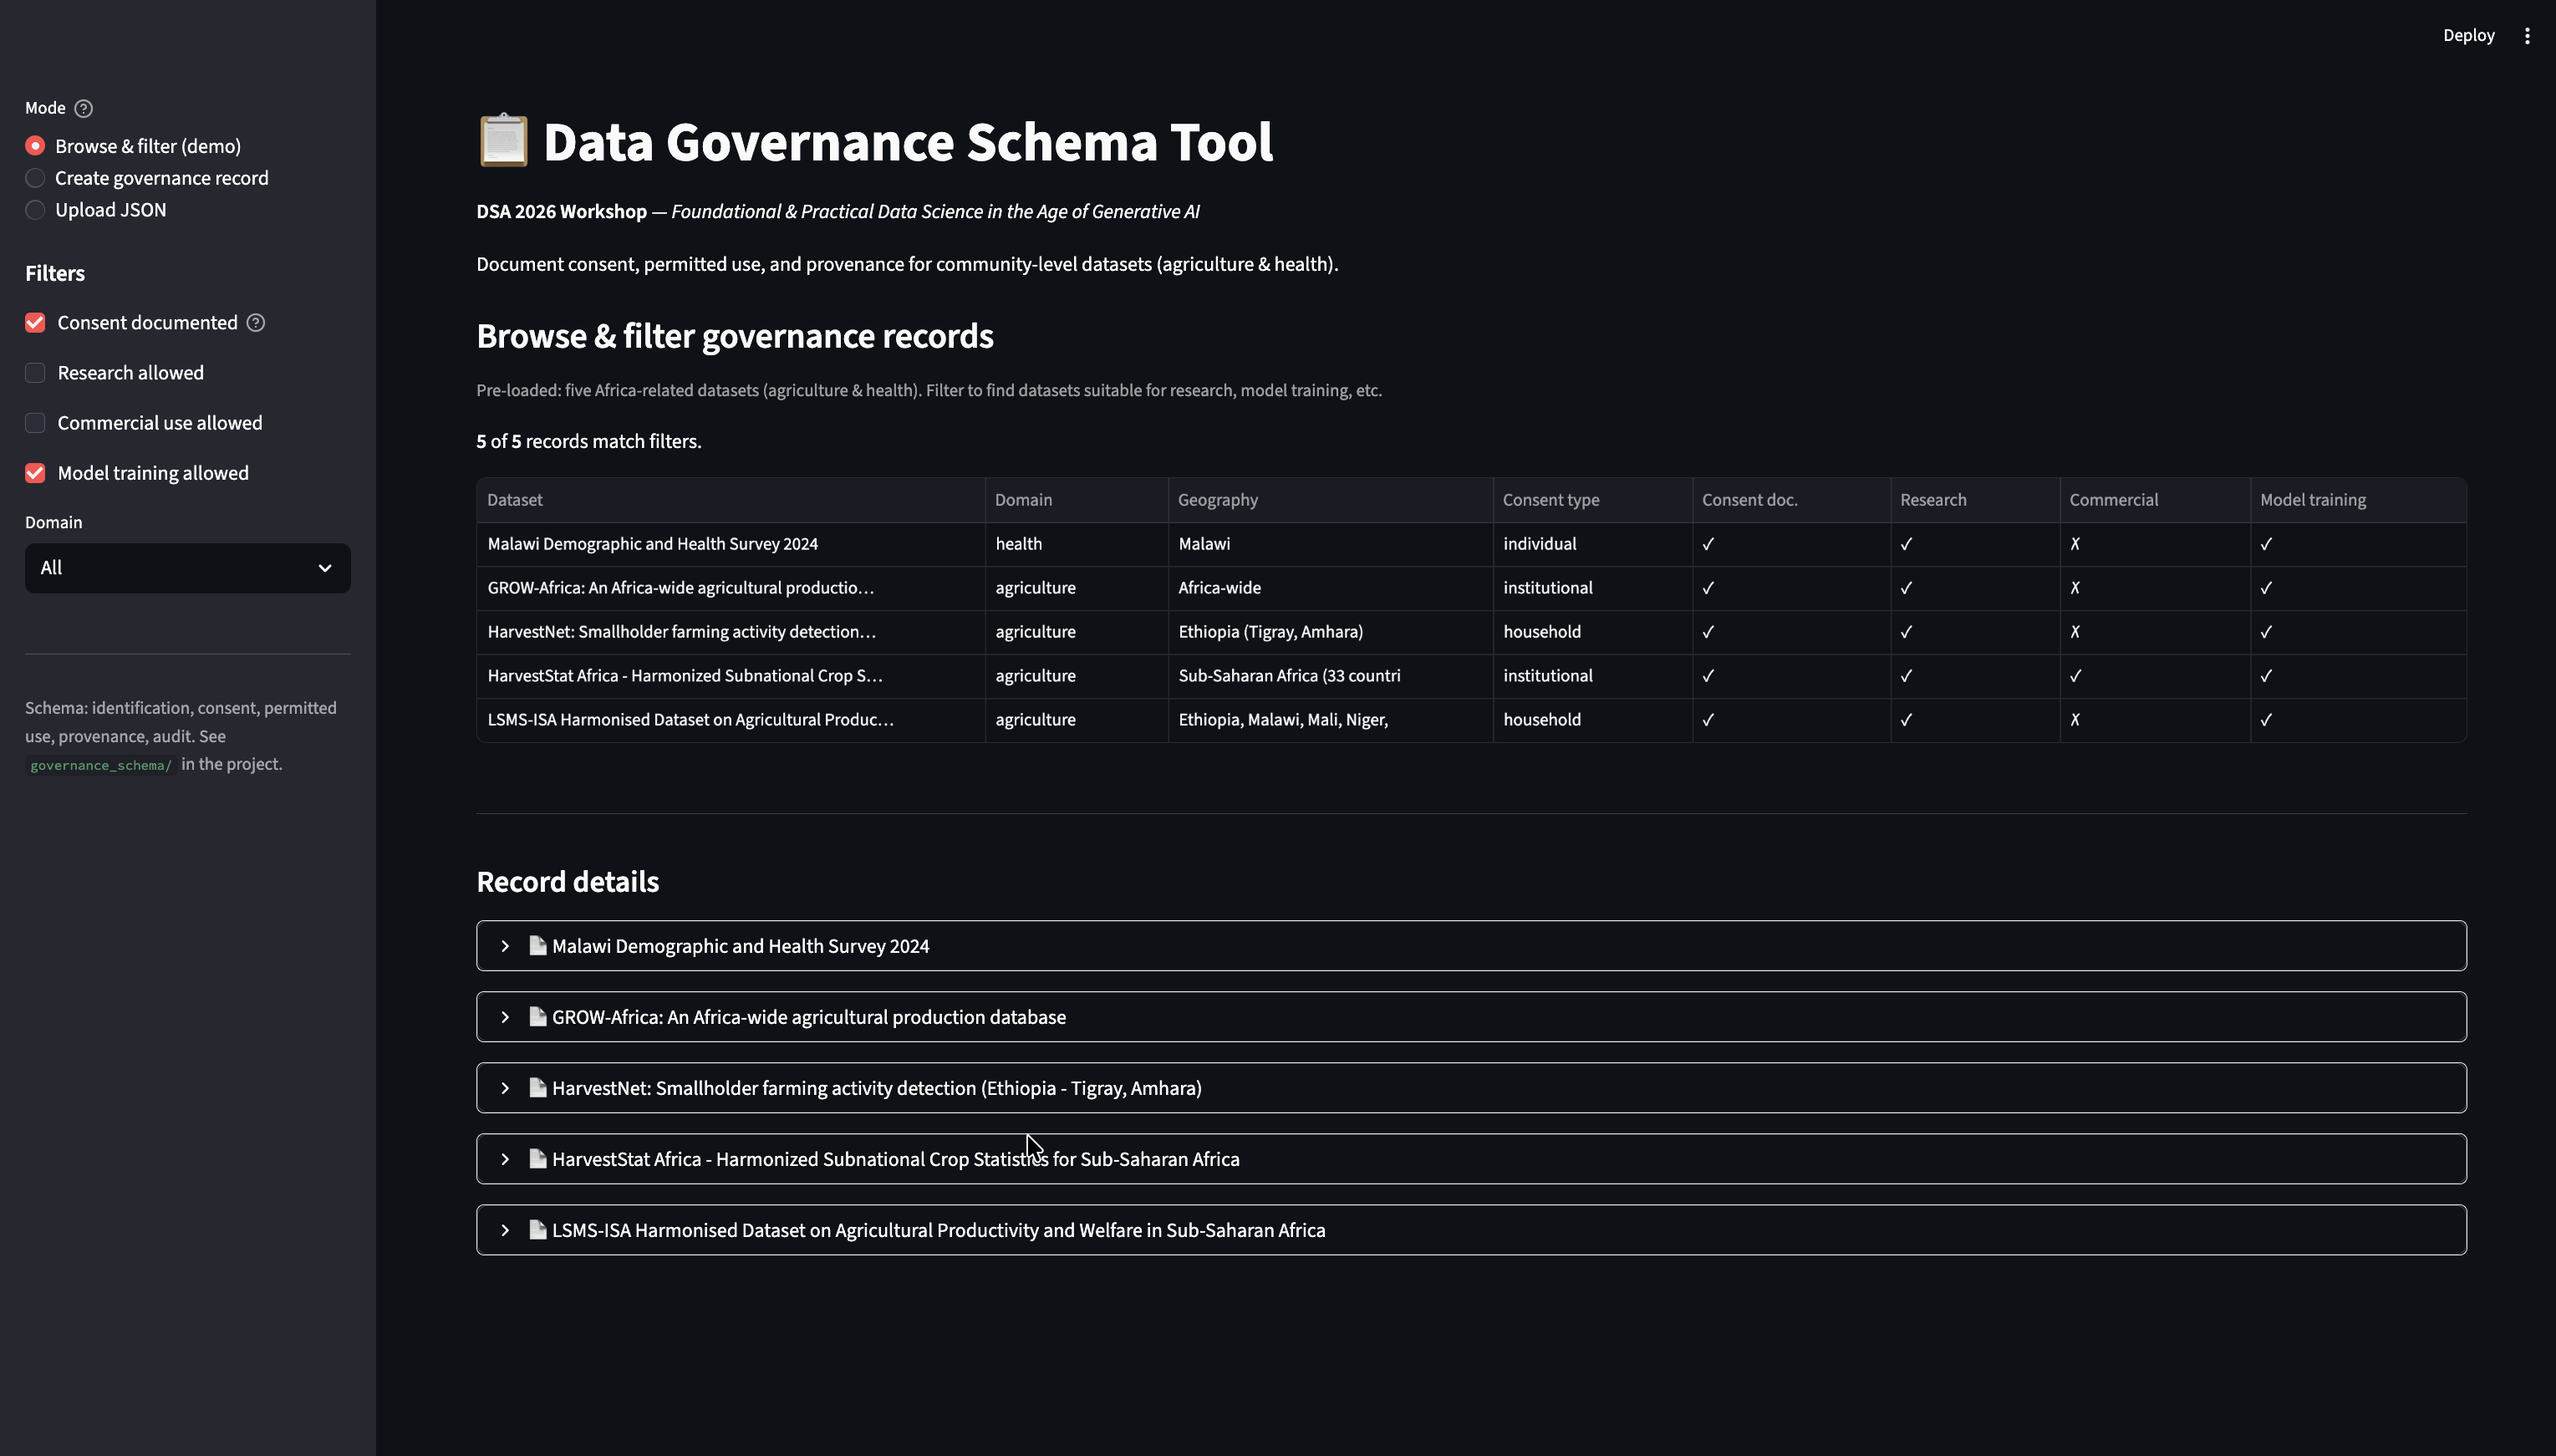
\includegraphics[width=\linewidth]{tool_screenshot_browse.png}
\small\textbf{(a)} Browse and filter governance records.
\end{minipage}
\hfill
\begin{minipage}{0.48\textwidth}
\centering
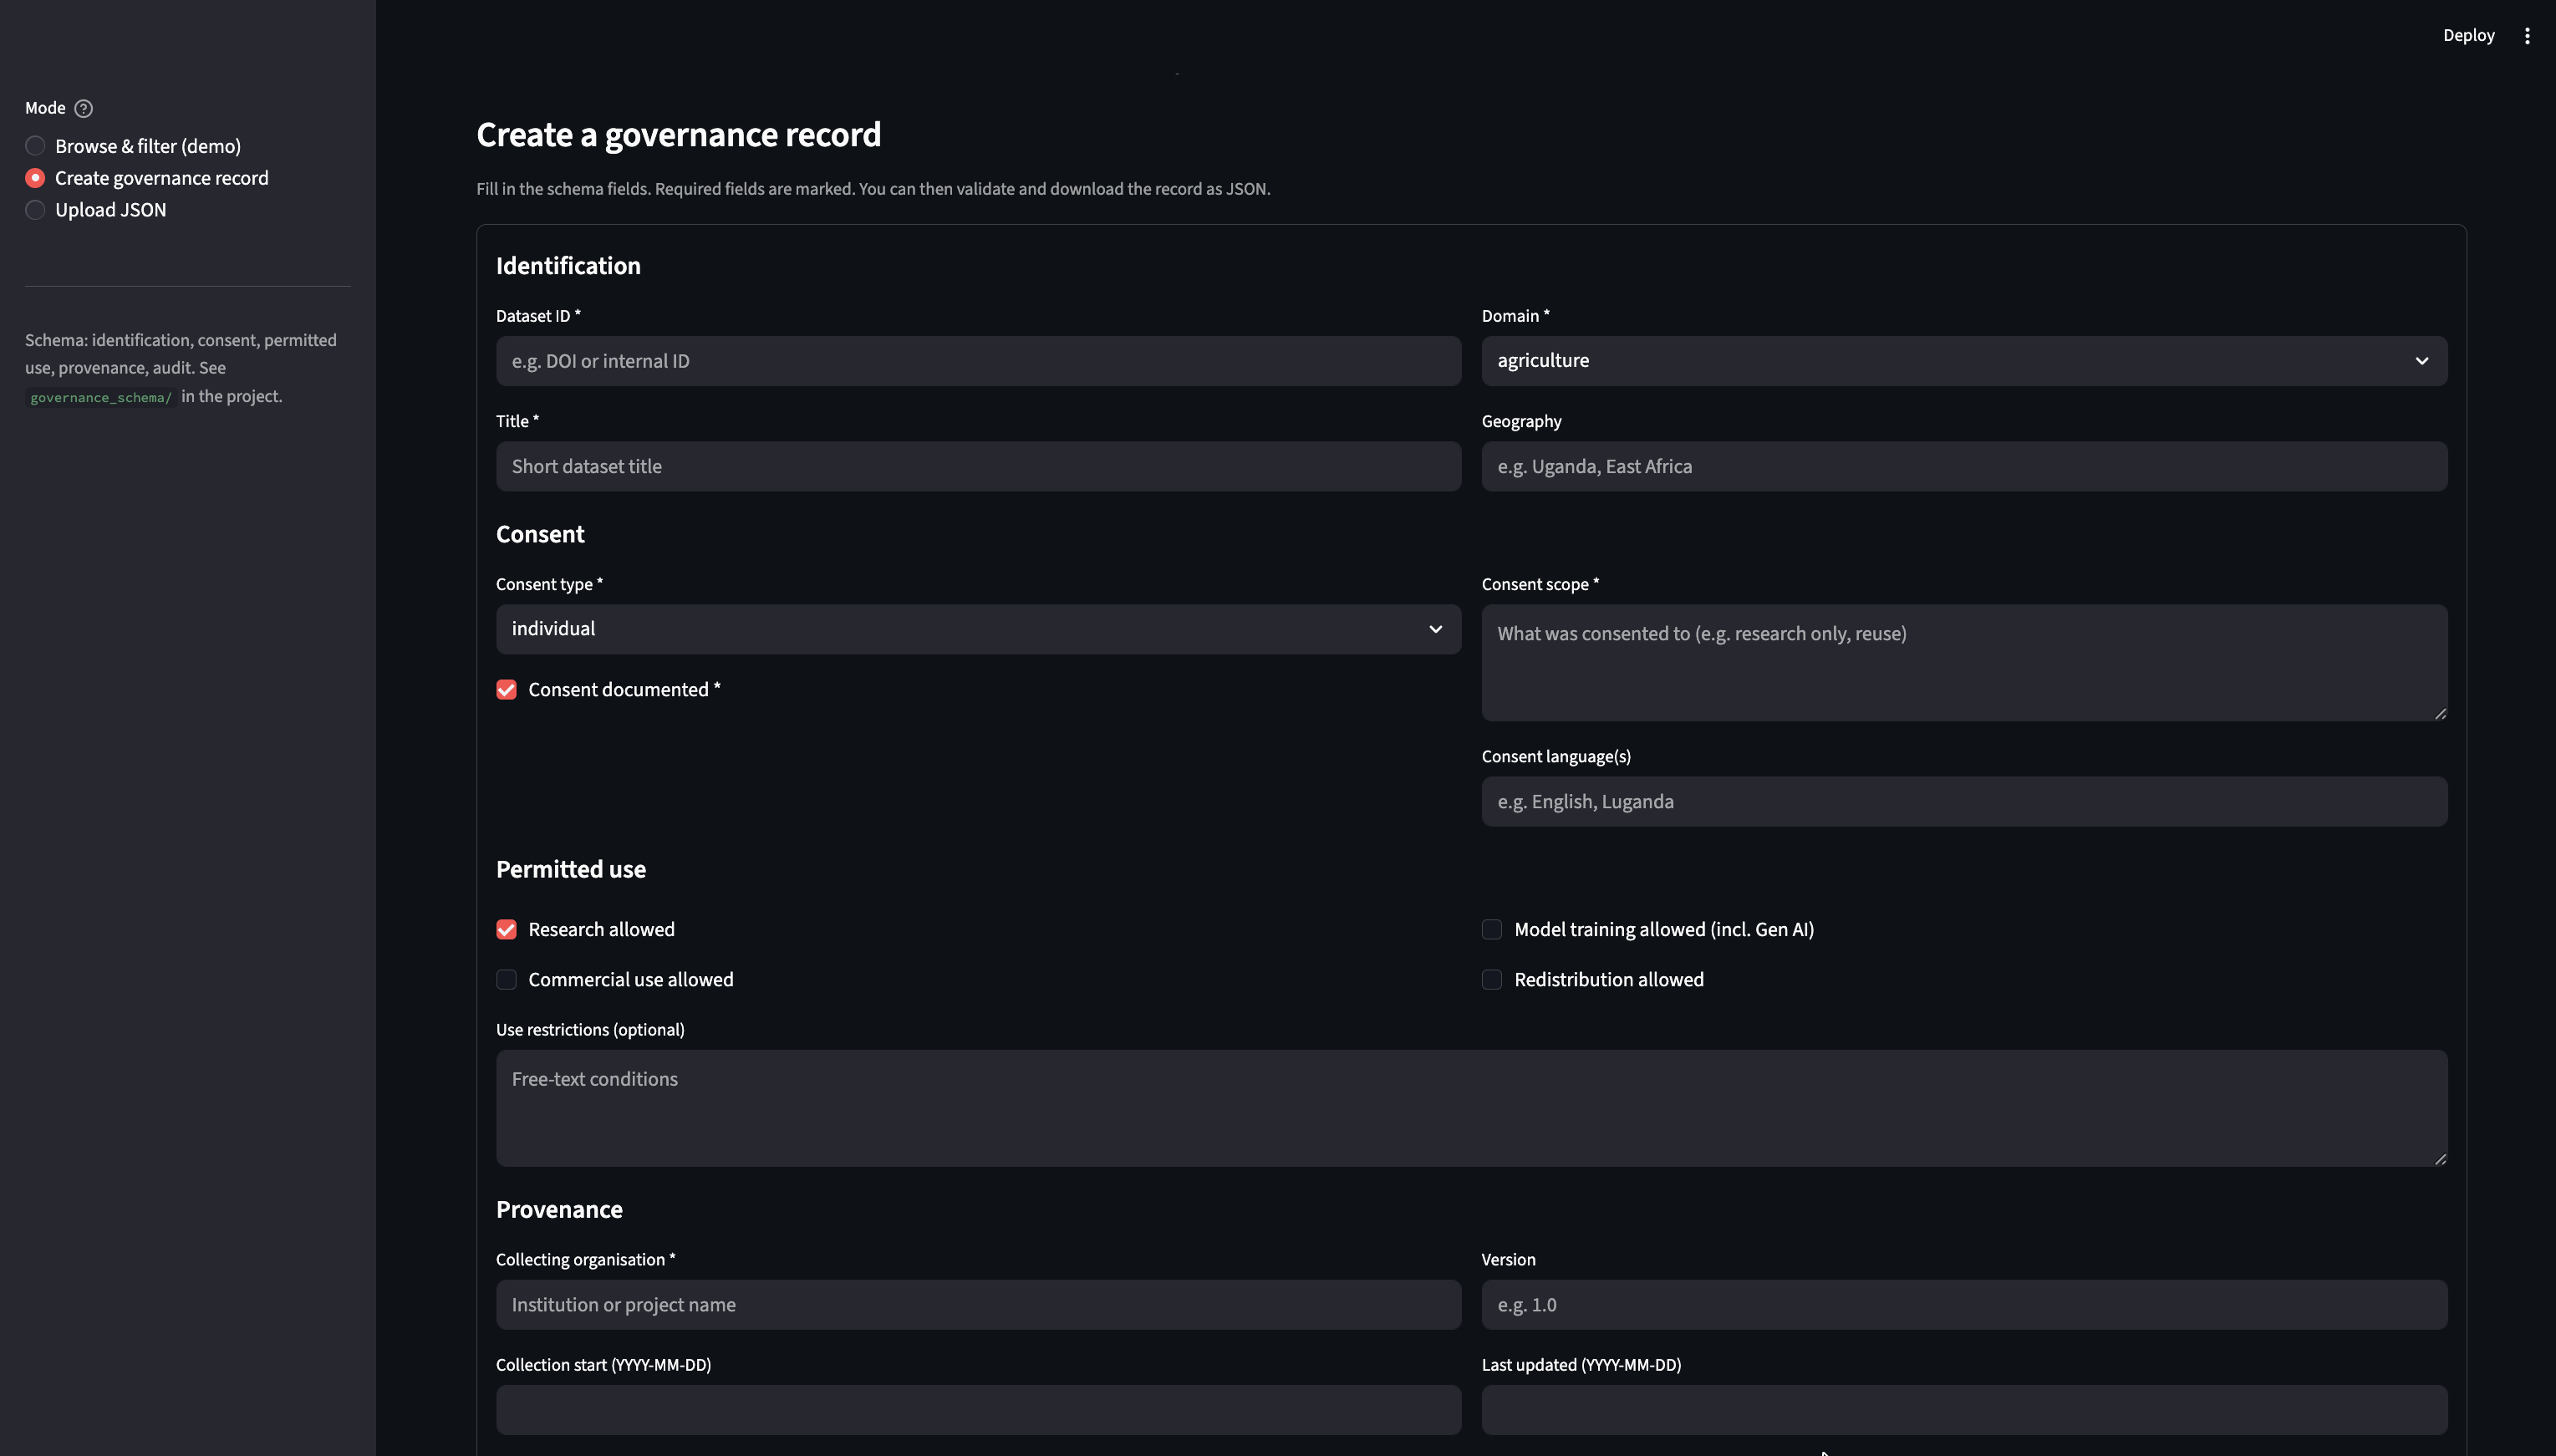
\includegraphics[width=\linewidth]{tool_screenshot_form.png}
\small\textbf{(b)} Create a new governance record.
\end{minipage}
\caption{Streamlit tool: (a) browsing and filtering the five governance records by domain, consent type, and permitted-use flags; (b) form for creating a new governance record with validation.}
\label{fig:tool}
\end{figure*}

\section{Application to Five Africa-Related Datasets}
\label{sec:application}

To demonstrate that the schema is expressive enough to capture real variation in governance practices, it was applied to five recent, publicly available, Africa-related datasets spanning agriculture, health, and remote sensing. For each dataset, a governance record was produced by consulting the official documentation, licence terms, and data-access procedures. The resulting records are summarised in Table~\ref{tab:application}.

\begin{table*}[t]
\centering
\caption{Application summary: five datasets and selected governance fields. Res.\ = research, Comm.\ = commercial, ML = model training, Redist.\ = redistribution, Doc.\ = consent documented.}
\label{tab:application}
\small
\begin{tabular}{@{}llllccccc@{}}
\toprule
Dataset & Domain & Geography & Consent & Res. & Comm. & ML & Redist. & Doc. \\
\midrule
HarvestStat Africa & Agriculture & SSA (33 countries) & Institutional & \checkmark & \checkmark & \checkmark & \checkmark & \checkmark \\
LSMS-ISA harmonised & Agriculture & 7 SSA countries & Household & \checkmark & $\times$ & \checkmark & $\times$ & \checkmark \\
GROW-Africa & Agriculture & Africa-wide & Institutional & \checkmark & $\times$ & \checkmark & $\times$ & \checkmark \\
Malawi DHS 2024 & Health & Malawi & Individual & \checkmark & $\times$ & \checkmark & $\times$ & \checkmark \\
HarvestNet (Ethiopia) & Agriculture & Ethiopia & Household & \checkmark & $\times$ & \checkmark & $\times$ & \checkmark \\
\bottomrule
\end{tabular}
\end{table*}

\paragraph{HarvestStat Africa.} This dataset \cite{desbureaux2025} provides harmonised subnational crop statistics covering 574,000 records across 33 sub-Saharan African countries. It is released under a CC0 (public-domain) licence. The governance record documents institutional consent (the data was assembled from national statistical offices), and all four permitted-use flags are set to true. This is the most permissive dataset in the sample.

\paragraph{LSMS-ISA harmonised.} The Living Standards Measurement Study -- Integrated Surveys on Agriculture \cite{gourlay2025} is a longitudinal household- and plot-level dataset spanning seven SSA countries from 2008 to 2024. Consent was obtained at the household level during enumeration. The World Bank's terms of use allow research and model training but prohibit commercial use and redistribution of microdata. The governance record captures this distinction, including a note in the \texttt{use\_restrictions} field about the requirement to agree to the World Bank's data-access terms.

\paragraph{GROW-Africa.} This Africa-wide database of crop yields \cite{jain2025} contains 535,000 observations assembled from multiple national and sub-national sources. The governance record reflects institutional consent (the data was compiled from official statistics), with research and model training allowed but commercial use and redistribution prohibited. The provenance section records the multi-source assembly process.

\paragraph{Malawi DHS 2024.} The Demographic and Health Survey for Malawi covers more than 22,000 households and includes detailed individual-level health, fertility, and nutrition indicators. Individual consent is documented and the DHS programme has robust governance: research and model training are allowed for registered projects, but commercial use and microdata redistribution are strictly prohibited. The governance record includes a note that DHS registration and data-use agreement are prerequisites.

\paragraph{HarvestNet (Ethiopia).} This smallholder dataset combines remote-sensing imagery with ground-truth crop labels collected from Ethiopian farmers. The governance record documents household-level consent and permits research and model training, but not commercial use or redistribution.

\subsection{Cross-Dataset Analysis}

Across the five records, the schema surfaces meaningful variation along multiple dimensions. Three consent types appear (institutional, household, individual), reflecting the heterogeneity of data-collection practices in African agriculture and health. Four of five datasets restrict commercial use and redistribution, suggesting that permissive open-data licences remain the exception rather than the rule for community-level data on the continent. All five datasets document consent and allow model training for research, which means a user searching for ``training data with documented consent'' would retrieve all five.

The schema supports three practical use cases. First, \textbf{filtering for ethical ML}: a researcher building a crop-yield model can select only datasets where consent is documented and model training is permitted, without manually reading each dataset's licence page. Second, \textbf{filtering by domain or geography}: a health-focused project can restrict to the DHS record, while a pan-African agriculture study can include HarvestStat, LSMS-ISA, and GROW-Africa. Third, \textbf{audit}: the provenance and audit fields answer ``who collected this, when, and who to contact,'' enabling compliance checks and due-diligence processes for institutional data users.

\section{Discussion}
\label{sec:discussion}

\subsection{Implications}

The schema is deliberately minimal and machine-readable, so it can sit alongside existing data-access policies \cite{effoduh2024} and support the kind of clear guidelines that health researchers in sub-Saharan Africa have asked for \cite{brown2024,chabilall2024}. By making consent and permitted use machine-readable, the schema lowers the governance barrier to responsible ML experimentation while preserving institutional control. A data collector who fills in a governance record does not cede any rights; the record simply makes existing terms visible and queryable.

Applying the schema to five diverse datasets shows that consent type and permitted use vary widely, from institutional to household to individual and from fully open (CC0) to restricted. Encoding these variations in a common format enables comparison, filtering, and audit across datasets that would otherwise require manual review of heterogeneous licence documents. This is particularly relevant in the context of generative AI, where large-scale data aggregation for model training often proceeds without granular attention to the governance status of individual datasets.

The dedicated \texttt{model\_training} flag addresses a gap in existing licence frameworks. Many datasets released before the current wave of foundation models use terms like ``research only'' without specifying whether model training counts as research. The schema forces an explicit answer to this question, reducing ambiguity for both data providers and consumers.

\subsection{Limitations}

Several limitations should be kept in mind. First, the five governance records were produced from publicly available documentation and terms of use; they have not been formally endorsed by the respective data custodians. Real-world adoption would require engagement with data providers to validate the records and integrate governance metadata into their distribution workflows.

Second, the schema documents governance conditions but does not enforce them. Enforcement remains with data custodians, institutional review boards, and legal frameworks. A user who ignores a ``commercial use prohibited'' flag faces no technical barrier from the schema itself. Future work could explore integration with access-control mechanisms or data-use agreements that enforce the flags programmatically.

Third, the schema has not yet been validated with data collectors or research ethics committees in Africa. Usability testing with community-level data collectors, particularly in low-resource and multilingual settings, would be an important next step. The Streamlit tool provides a starting point, but it assumes internet access and English literacy, which may not hold in all collection contexts.

Fourth, the taxonomy of consent types (individual, community, household, institutional) is necessarily a simplification. Real consent processes are often layered (e.g.\ community permission followed by individual opt-in) and may evolve over time. The schema captures the primary consent type but cannot represent the full complexity of consent negotiations in every context.

\subsection{Future Work}

Future work could extend the Streamlit application into a hosted service for data collectors, potentially with offline support and multilingual interfaces. Aligning the schema more closely with African data ethics frameworks \cite{barrett2025} and data justice principles \cite{munung2025} could strengthen its normative grounding. Running adoption pilots with one or two African research institutions would test whether the schema is practical in real data-collection workflows. Finally, adding optional fields for data retention, data minimisation, or benefit-sharing terms could accommodate evolving regulatory requirements across African jurisdictions.

\section{Conclusion}

This paper introduced a minimal governance schema for community-level datasets that records consent type and scope, permitted use (research, commercial, model training, redistribution), and provenance and audit information. The schema was applied to five recent Africa-related datasets in agriculture and health, and the results show that it surfaces meaningful variation in consent practices and permitted use, supporting filtering for ethical downstream ML and audit trails. The schema, template, filled records, and Streamlit tool are offered as a reusable artefact for practical data governance in the age of generative AI, where reuse and training on community data ought to be traceable and consent-aware.

\section*{Ethical Statement}

This work proposes a governance schema for documenting consent and permitted use of community-level datasets. No human subjects were involved in this study. The five governance records were produced from publicly available dataset documentation and terms of use; no private or restricted data was accessed. The schema is intended to support ethical data practices by making consent and permitted use visible and queryable. It does not replace institutional review, legal compliance, or community engagement, all of which remain essential for responsible data governance. The authors recognise that governance schemas can be misused (e.g.\ to create a false impression of compliance), and emphasise that the schema documents conditions as stated by data providers; independent verification remains necessary.

\bibliographystyle{named}
\bibliography{references}

\end{document}
